\documentclass[10pt,twocolumn]{article}

\usepackage[margin=0.75in]{geometry}
\usepackage{times}
\renewcommand{\ttdefault}{cmtt}
\usepackage{graphicx}
\usepackage{booktabs}
\usepackage{amsmath}
\usepackage{natbib}
\usepackage[hidelinks]{hyperref}
\usepackage{url}
\usepackage{listings}

\lstdefinestyle{promptbox}{
  basicstyle=\ttfamily\scriptsize,
  breaklines=true,
  breakatwhitespace=false,
  columns=fullflexible,
  keepspaces=true,
  showstringspaces=false,
  frame=single,
  framerule=0.4pt,
  xleftmargin=0pt,
  xrightmargin=0pt,
  aboveskip=5pt,
  belowskip=9pt
}

\urlstyle{same}
\sloppy
\raggedbottom

\title{El Agente Creativo: Agentic Generation of Research Ideas with Representation Networks}
\author{Anonymous authors}

\begin{document}
\maketitle

\begin{abstract}
We disentangle the contributions of explicit literature structure
from those of the agentic loop in LLM research ideation.  \textbf{El
Agente Creativo} composes ideas by traversing a representation network
distilled from source papers; a matched \textbf{Abstracts agent} baseline
shares its LLM, workflow, output schema, and tool-call budget but
reasons over the flat abstract corpus.  Using an LLM-as-judge Elo
protocol calibrated on ICLR oral-vs-poster gaps, we find that both
agentic arms beat a deliberately strong shuffled LLM-only baseline by
$57$--$123$ Elo and exceed an ICLR 2026 oral anchor, yet tie each
other on quality---the headline gain is carried by the agentic loop,
not by graph structure per se.  Graph structure instead delivers a
consistent nearest-neighbor diversity edge, largest cross-domain, at
$1.29$--$1.79\times$ lower per-idea token cost.  Schema-isolating
ablations trace this edge to the typed Repr/Transform schema: ReprNet
beats a matched generic knowledge-graph agent by $+28.76$ to $+39.34$
Elo at matched cost, and removing the realization (is-a) hierarchy
erases most of the gap.  Agentic ideation is the right substrate; a
typed schema with an abstraction hierarchy is a consistent
diversity-and-cost win on top of it, most impactful when ideas must
bridge unfamiliar domains.
\end{abstract}

\section{Introduction}

Large language models (LLMs) are increasingly capable partners in the
scientific workflow, generating idea-like abstracts that read fluently and
recover surface markers of novelty
\citep{si2024llmsgeneratenovelresearch,kumar2025largelanguagemodelsunlock,lu2024aiscientistfullyautomated,vaswani2023attentionneed,brown2020languagemodelsfewshotlearners}.
This progress, however, has been measured almost entirely by whether the
output looks plausible, leaving open the question that matters for the
design of practical scientific assistants: given a fixed set of source
papers, does providing the LLM with a structured representation of the
literature actually produce better ideas than letting the same model read
the same abstracts directly?

This counterfactual is hard to answer because the obvious comparison is
biased against the LLM-only baseline.  If the LLM-only arm always sees source
abstracts in the same order, it can be penalized by positional artifacts
rather than by representation; if the two arms see different source pools,
quality differences can be attributed to the pool rather than to structure.
A genuine test of explicit structure therefore requires identical source
identities, controlled abstract order, and a quality judge whose scale is
itself externally validated---three constraints that have not been combined
in prior ideation benchmarks.

We address this gap with \textbf{El Agente Creativo}, a graph-conditioned
ideation agent that operates over a representation network in which each
source paper is distilled into a small set of reusable \emph{representation}
nodes and \emph{transform} nodes joined by typed edges, and that composes
new ideas by bridging these nodes through retrieval and traversal tools.
The agent is benchmarked against a deliberately strengthened LLM-only
baseline: the same LLM, given the \emph{same} source abstracts, with
abstract order deterministically reshuffled per generated idea so that no
fixed positional ordering can favor either arm.  Across both
within-domain (random ICLR) and cross-domain (Nature+ICLR) settings, this
controls the counterfactual at the level of source identity, abstract
ordering, and generation budget.

We pair this design with a calibration step that grounds the LLM-as-judge
evaluator in a known-quality signal.  Because LLM-as-judge tournaments are
sensitive to prompt and judge bias, we precede every generated-idea claim
with an oral-vs-poster calibration drawn from ICLR 2025 and ICLR 2026,
recovering 66.0 and 35.1 Elo gaps that anchor an interpretive reference
scale.  All idea-quality comparisons in the paper are reported against
this scale rather than as standalone Elo deltas, so the magnitude of the
effect can be interpreted directly.

The study makes four contributions.
\textbf{(i) Matched-source benchmarks.}  We construct random10 and
random20 ICLR 2025 benchmarks and an interdisciplinary Nature+ICLR
benchmark in which LLM-only and ReprNet agents generate ideas from identical
source-paper IDs and deterministically reshuffled abstract orders.
\textbf{(ii) Calibrated quality evaluation.}  We calibrate the Elo judge
on oral-vs-poster distinctions, recovering 66.0 and 35.1 Elo gaps, and use
these as an interpretive reference for generated-idea comparisons.
\textbf{(iii) Consistent quality and diversity gains.}  Graph-conditioned
ideation improves mean Elo by 111.7--151.0 points across all three
benchmarks, increases nearest-neighbor diversity in every setting, and
exceeds the ICLR 2026 oral anchor in two of three tournaments.
\textbf{(iv) End-to-end token observability.}  We instrument every
generation, traversal, and evaluation call, revealing that the ReprNet agent
spends 43--95$\times$ more tokens per idea, concentrated in input-side
traversal context rather than longer outputs, and identifying the most
impactful direction for follow-on engineering.

\section{Related Work}

\paragraph{LLM-based research ideation.}
Prior ideation benchmarks have measured what LLMs can produce but not
whether literature representation matters.  Recent studies show that
LLM-generated ideas can rival human-written proposals on novelty while
still trailing on feasibility, grounding, and diversity
\citep{si2024llmsgeneratenovelresearch,kumar2025largelanguagemodelsunlock};
IdeaBench supplies target-paper and reference-paper contexts for
biomedical ideation, and AI Idea Bench scales the protocol to AI papers
across multiple evaluation views
\citep{guo2025ideabench,qiu2025aiideabench}.  These efforts motivate our
matched-source protocol, but none isolates the causal effect of the
underlying literature representation.  El Agente Creativo is designed
specifically to ask the narrower counterfactual question: does a graph
view of the same papers improve generation over flat prompting?

\paragraph{Structured representations for ideation.}
A growing literature already pre-structures the literature before
ideation, but none of these systems isolates the representation effect.
SciMON optimizes scientific inspirations for novelty, SciDeator recombines
research-paper facets, and Idea-Catalyst decomposes research problems
before retrieving and ranking cross-domain source insights
\citep{wang2024scimon,radensky2024scideator,kargupta2026ideacatalyst}.  In
parallel, knowledge-grounded and agentic discovery systems---KG-CoI,
SciAgents, The AI Scientist, and Robin---wire graphs, tool use, or
multi-agent loops into broader hypothesis-generation workflows
\citep{xiong2024kgcoi,ghafarollahi2024sciagents,lu2024aiscientistfullyautomated,ghareeb2025robin}.
El Agente Creativo is complementary to these systems: rather than building
a full discovery agent, it isolates the representation layer and benchmarks
graph-conditioned ideation head-to-head against a shuffled-abstract
baseline that holds the source pool identical.

\paragraph{Evaluation methodology.}
Evaluation choices materially shape what one can claim about generated
science, and existing protocols do not provide a calibrated scale.
OpenNovelty grounds novelty assessment in retrieved supporting evidence,
and ScholarEval targets literature-grounded research-idea evaluation
\citep{zhang2026opennovelty,moussa2025scholareval}.  Our protocol is
lighter-weight than a full novelty audit but adds two features tailored to
the present question: a calibration step that recovers the ICLR
oral-vs-poster gap before any generated-idea claim is made, and per-call
token observability that exposes the quality--cost tradeoff hidden inside
agent pipelines.

\section{The El Agente Creativo Pipeline}

El Agente Creativo decouples scientific ideation into two stages so that explicit
representation can be evaluated as an isolated design choice.  In
\emph{graph construction}, each source paper is distilled into a compact
set of representation nodes, transform nodes, and typed edges, with an
extraction prompt that is budget-constrained so that each paper contributes
its core contribution as a reusable abstraction rather than as verbatim
transcription.  In \emph{graph-conditioned ideation}, an LLM agent
traverses the resulting network through retrieval and traversal
tools---sampling random nodes, expanding parent and child hierarchies,
finding paths between distant concepts---and returns a single paper-style
idea per run.

The LLM-only baseline preserves every degree of freedom except the
representation.  It receives the same source papers as plain text under
deterministically reshuffled abstract order, returns an idea under the
identical JSON schema, and shares the underlying LLM and decoding settings
with the ReprNet agent.  The only systematic difference between the two arms
is whether the model interacts with the literature through a graph or
through a flat list of abstracts.

A central design invariant is that prior experiment graphs are treated
as read-only artifacts so that quality gains cannot be confounded by
silent graph mutation.  Every reuse of a cached graph proceeds through
an experiment-scoped duplicate whose contents are verified against the
source by SHA-256 fingerprints over node and edge payloads; the
duplication and verification mechanics are described in
Appendix~\ref{app:method-details} (Figure~\ref{fig:pipeline}).

\begin{figure*}[t]
  \centering
  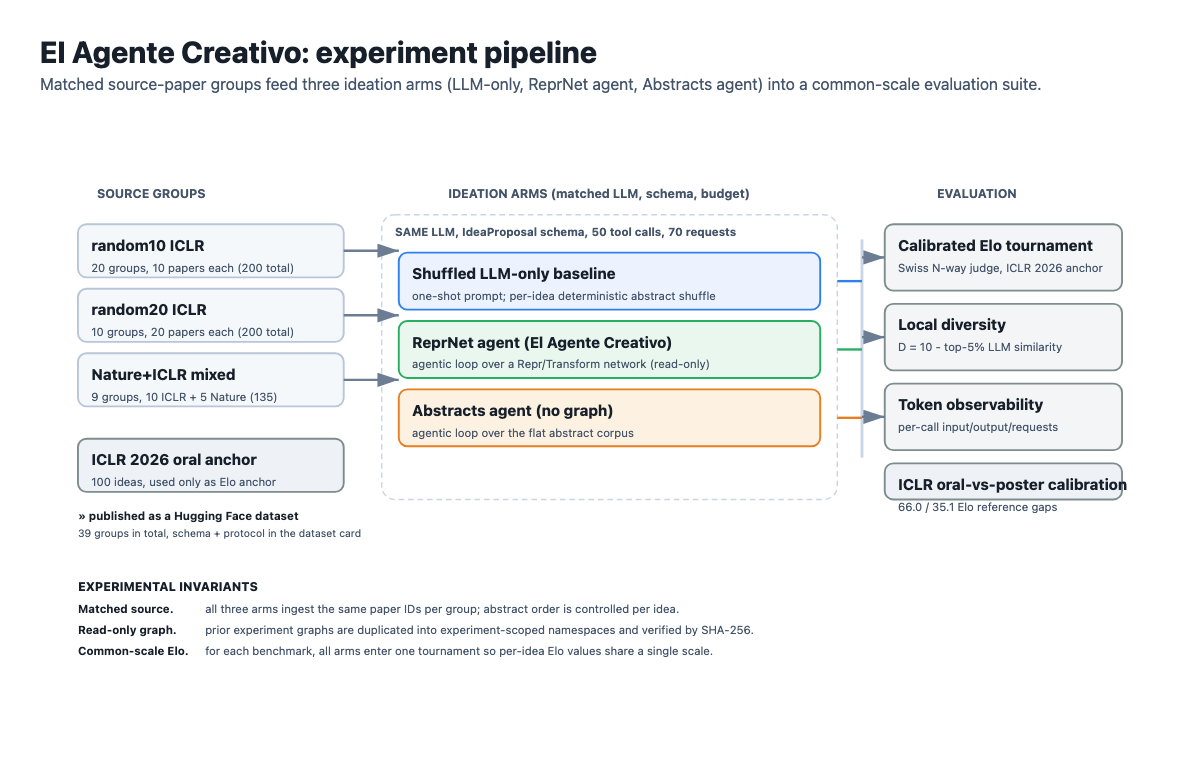
\includegraphics[width=0.92\textwidth]{figures/fig_pipeline.png}
  \caption{End-to-end experiment pipeline.  Source paper abstracts are
  split into matched groups; the shuffled LLM-only baseline (top), the
  ReprNet agent (middle, reusing read-only representation networks from a
  prior run), and the Abstracts agent baseline (right of middle) each
  generate ideas from the \emph{same} groups under matched LLM,
  schema, and tool-call budgets; outputs feed a unified Elo
  tournament, a nearest-neighbor diversity evaluator, and a per-call
  token-observability log.}
  \label{fig:pipeline}
\end{figure*}

\section{Experimental Design}

\paragraph{Judge calibration.}
Every generated-idea claim in this paper is preceded by an oral-vs-poster
calibration so that the Elo scale is externally validated before it is used
to compare arms.  The same Elo protocol is run over 100 ICLR 2025 oral
abstracts versus 100 poster abstracts, and independently over the
corresponding ICLR 2026 split, yielding two reference gaps against which
all subsequent quality differences are read.

\paragraph{Matched random ICLR benchmark.}
The primary benchmark holds source identity constant across arms while
sampling without submission-side filtering bias.  Its source pool
consists of 600 accepted ICLR 2025 papers obtained from OpenReview by
querying accepted-venue counts with random offsets, partitioned into
twenty disjoint random10 groups (primary condition) and ten disjoint
random20 groups (secondary condition); each group produces ten LLM-only
ideas and ten ReprNet-agent ideas.  Abstract order is shuffled per idea with a
deterministic seed so the LLM-only arm cannot be penalized by a fixed
positional artifact, and the ReprNet agent reuses cached graphs through a
fingerprint-verified read-only duplicate
(Appendix~\ref{app:method-details}).

\paragraph{Abstracts agent (non-graph agentic baseline).}
To distinguish the contribution of explicit graph structure from that
of the agentic loop, every benchmark in this paper also includes a
third arm called \textbf{Abstracts agent}.  Abstracts agent shares every degree of
freedom with the ReprNet agent (same LLM, same Pydantic AI framework, same
\texttt{IdeaProposal} schema, same source IDs, same 50 tool-call and
70 request budget, same workflow of sample $\to$ inspect $\to$ explore
neighbors $\to$ bridge $\to$ synthesize $\to$ self-critique) but its
tool palette (\texttt{random\_paper}, \texttt{read\_paper},
\texttt{search\_papers}, \texttt{find\_related}, \texttt{bridge}) acts
on the flat abstract corpus rather than on the representation graph,
using sentence-embedding cosine similarity in place of typed-edge
traversal.  Abstracts agent generates 10 ideas per group at each
benchmark---200 at random10, 100 at random20, 90 at Nature+ICLR
mixed---and enters the tournament for each setting alongside the
LLM-only, ReprNet-agent, and (where applicable) ICLR 2026 oral anchor pools.
Half-budget Elo tournaments (1200 matches for random10, 2400 for
random20, 1800 for mixed) are used because the addition of a fourth
arm doubles compute relative to the original two-arm V2 measurements;
this leaves rms convergence below 10 Elo in all cases, sufficient to
read the ReprNet-vs-Abstracts comparisons.  The interdisciplinary
methodology for the mixed setting mirrors the ReprNet agent's mixed
methodology so both agentic arms face the same cross-domain
constraints.

\paragraph{Interdisciplinary Nature+ICLR benchmark.}
A second benchmark tests whether the effect transfers to a genuinely
cross-disciplinary setting where domain integration is the central
challenge.  It uses nine mixed groups, each starting from an ICLR
random10 graph and augmented with five recent Nature-family abstracts
spanning Nature Physics, Nature Biotechnology, and Nature Chemistry;
LLM-only and ReprNet agents each generate ten ideas per group.  Beyond Elo
and diversity, a dedicated rubric scores each idea on five
interdisciplinarity axes---domain coverage, integration depth,
bidirectional value, source grounding, and feasibility---on a 1--5
scale.

\section{Evaluation Methodology}

\subsection{Quality via Calibrated Elo}

Idea quality is scored by a blinded LLM-as-judge tournament whose
pairwise preferences drive a Bradley--Terry update over per-idea Elo
ratings \citep{elo1978rating,bradley1952rank}.  All ideas in a setting
begin at Elo 1000; each match presents $m=4$ ideas chosen by a
Swiss-style scheduler that balances participant exposure, prefers
nearby Elo ratings after a warm-up phase, and retains an exploration
term so mid-rank pairings remain well sampled
\citep{zheng2023judgingllmasajudgemtbenchchatbot,chiang2024chatbotarenaopenplatform};
presentation order is shuffled before judging.  The judge returns a
complete ranking which is decomposed into all $m(m-1)/2$ pairwise
comparisons and applied via the standard Bradley--Terry expected-score
update with $K=32$ (see Appendix~\ref{app:method-details} for the
exact equations).  The reported quality score for each arm is its mean
final Elo, with nonparametric bootstrap 95\% confidence intervals over
idea-level Elo values.  Because the same protocol is first applied to
oral-vs-poster calibration sets, every generated-idea gap is read
against a known-quality reference scale rather than as an isolated
number.

\subsection{Local Diversity}

A second axis is required because Elo can reward a base of near-duplicate
ideas without penalty.  We therefore measure \emph{local self-similarity}
inside each idea base: for every idea, we embed its title and abstract,
retrieve the top 5\% nearest neighbors by cosine similarity, deduplicate
pairs, and cap the evaluation at the configured budget, after which an LLM
rates each pair on a 1--10 semantic-similarity scale.  Following the
spirit of Self-BLEU-style redundancy checks \citep{zhu2018texygen}, we
report
\begin{equation}
  D = 10 - \frac{1}{|\mathcal{P}|}\sum_{(i,j)\in\mathcal{P}} s(i,j),
\end{equation}
where $\mathcal{P}$ is the selected nearest-neighbor pair set and
$s(i,j)$ the LLM similarity score; higher $D$ corresponds to lower local
redundancy.  Because nearest-neighbor diversity is sensitive to
source-set breadth, $D$ is always interpreted jointly with Elo rather
than as a stand-alone metric.

\subsection{Token Observability}

A third axis records the cost incurred to produce the quality and
diversity signals so the tradeoff is auditable rather than implicit.
Every generated idea and every judge call logs normalized input,
output, and request counts; the five expenditure categories (graph
construction, graph traversal, Elo judging, diversity judging, and
rubric judging) are reported separately because their cost profiles
differ qualitatively.  The full normalization conventions and per-step
totals are deferred to Appendix~\ref{app:method-details}
(Table~\ref{tab:stepcost}).

\section{Results}
\label{sec:results}

\subsection{The Judge Recovers a Known Quality Distinction}

The Elo protocol reliably recovers the externally validated ICLR
oral-vs-poster ranking in two independent calibration tournaments
(Figure~\ref{fig:calibration}).  ICLR 2025 oral ideas reach a mean Elo of
1033.0 versus 967.0 for posters, a 66.0 Elo gap; ICLR 2026 oral ideas reach
1017.6 versus 982.5 for posters, a 35.1 Elo gap.  These two values do not
claim to capture absolute scientific merit, but they do establish that the
protocol is sensitive to a known venue-quality distinction, and they fix
the interpretive scale for the generated-idea comparisons that follow.

\begin{figure*}[t]
  \centering
  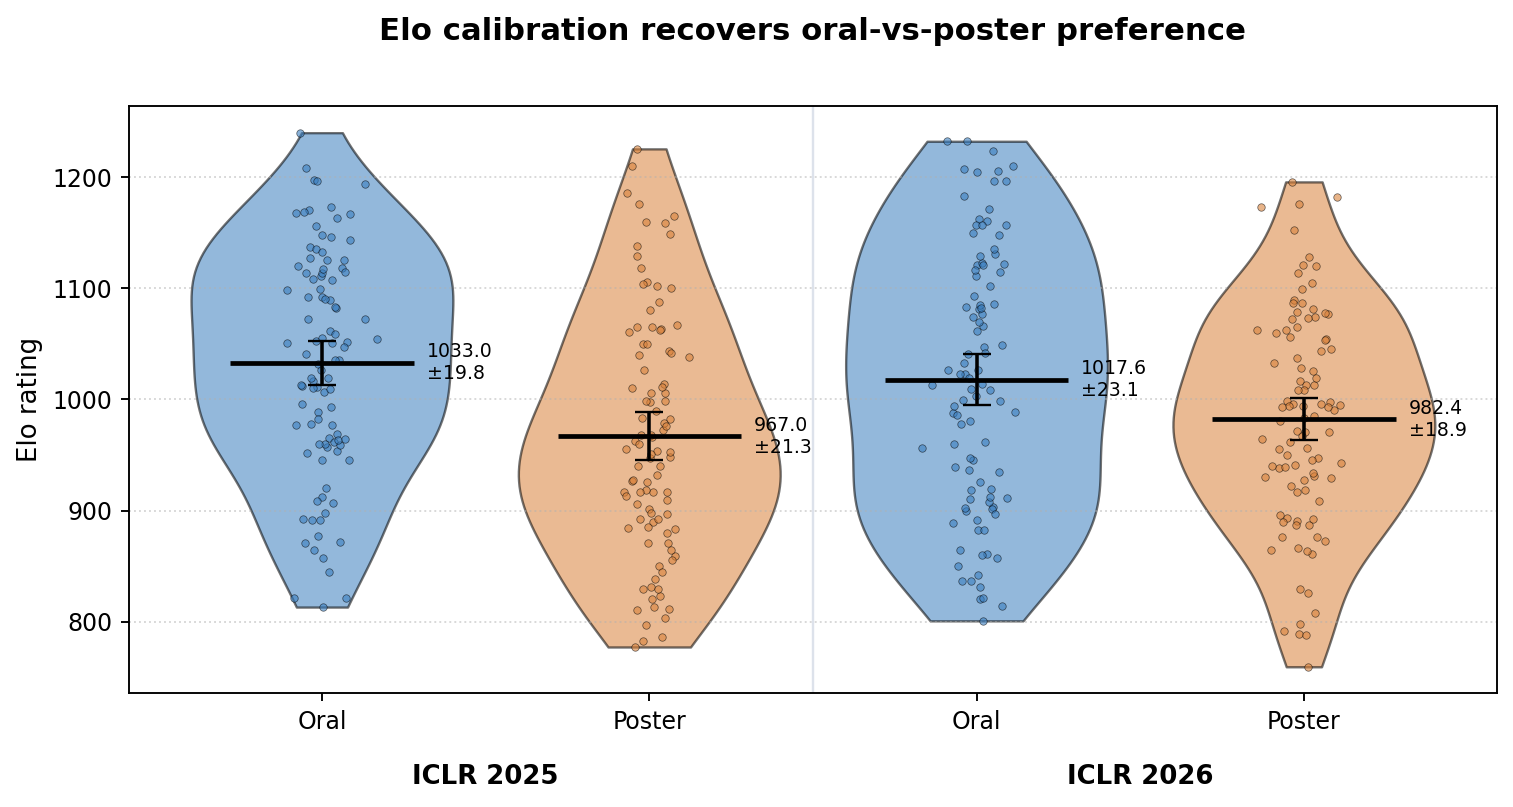
\includegraphics[width=0.7\textwidth]{figures/fig_calibration.png}
  \caption{Calibration: the Elo judge separates ICLR oral abstracts
  from poster abstracts by $66.0$ Elo on the 2025 split and $35.1$ Elo
  on the 2026 split, recovering the externally known venue-quality
  ordering.  Violins show per-idea Elo distributions; rules and error
  bars are means with $\pm 1.96 \cdot \mathrm{SEM}$ 95\% confidence
  intervals.  These two gaps anchor the interpretive reference scale
  for every subsequent generated-idea comparison.}
  \label{fig:calibration}
\end{figure*}

\begin{table}[t]
\centering
\small
\begin{tabular}{lrrrr}
\toprule
Set & Poster Elo & Oral Elo & Gap & Matches \\
\midrule
ICLR 2025 & 967.0 & 1033.0 & 66.0 & 1000 \\
ICLR 2026 & 982.5 & 1017.6 & 35.1 & 1000 \\
\bottomrule
\end{tabular}
\caption{Oral-vs-poster calibration.  The gap is oral minus poster mean Elo.}
\label{tab:calibration}
\end{table}

\subsection{Agentic Ideation Beats LLM-only Across All Settings; ReprNet and Abstracts Agents Tie on Quality}

Both agentic arms improve mean Elo by $+56.8$ to $+123.0$ points over
the shuffled LLM-only baseline across all three benchmarks
(Table~\ref{tab:quality}, Figure~\ref{fig:quality}); the gap exceeds
the calibrated oral-vs-poster reference (66.0 and 35.1 Elo) in every
setting and surpasses the ICLR 2026 oral anchor in both random-ICLR
tournaments.  When the ReprNet and Abstracts agents are compared against each other
in a single common-scale tournament per setting, however, the two
arms are statistically indistinguishable on quality at every
benchmark: $+5.4$ Elo at random10 (tournament rms $\approx 5.8$),
$-0.8$ Elo at random20 (rms $\approx 7$), and $-7.8$ Elo at the
Nature+ICLR mixed setting (rms $\approx 8.2$).  The entire
agentic-vs-LLM-only advantage is therefore carried by the agentic loop
itself---iterative tool use, deliberation, and self-critique over a
30--35-call budget---rather than by the representation graph.

The shape of the agentic gap is itself informative.  In random10, the
agentic advantage over LLM-only is smallest ($+56.8$ Elo); in random20
it is largest ($+123.0$); in the cross-domain mixed setting it sits in
between ($+93.5$).  This nonmonotonic pattern is consistent with the
agentic loop benefitting most when each idea has a moderately broad
source context (random20's 20-paper pool) and proportionally less when
the pool is narrower (random10) or harder (mixed); the ReprNet agent adds no
further quality lift on top of this trend at the matched budget.

\begin{figure*}[t]
  \centering
  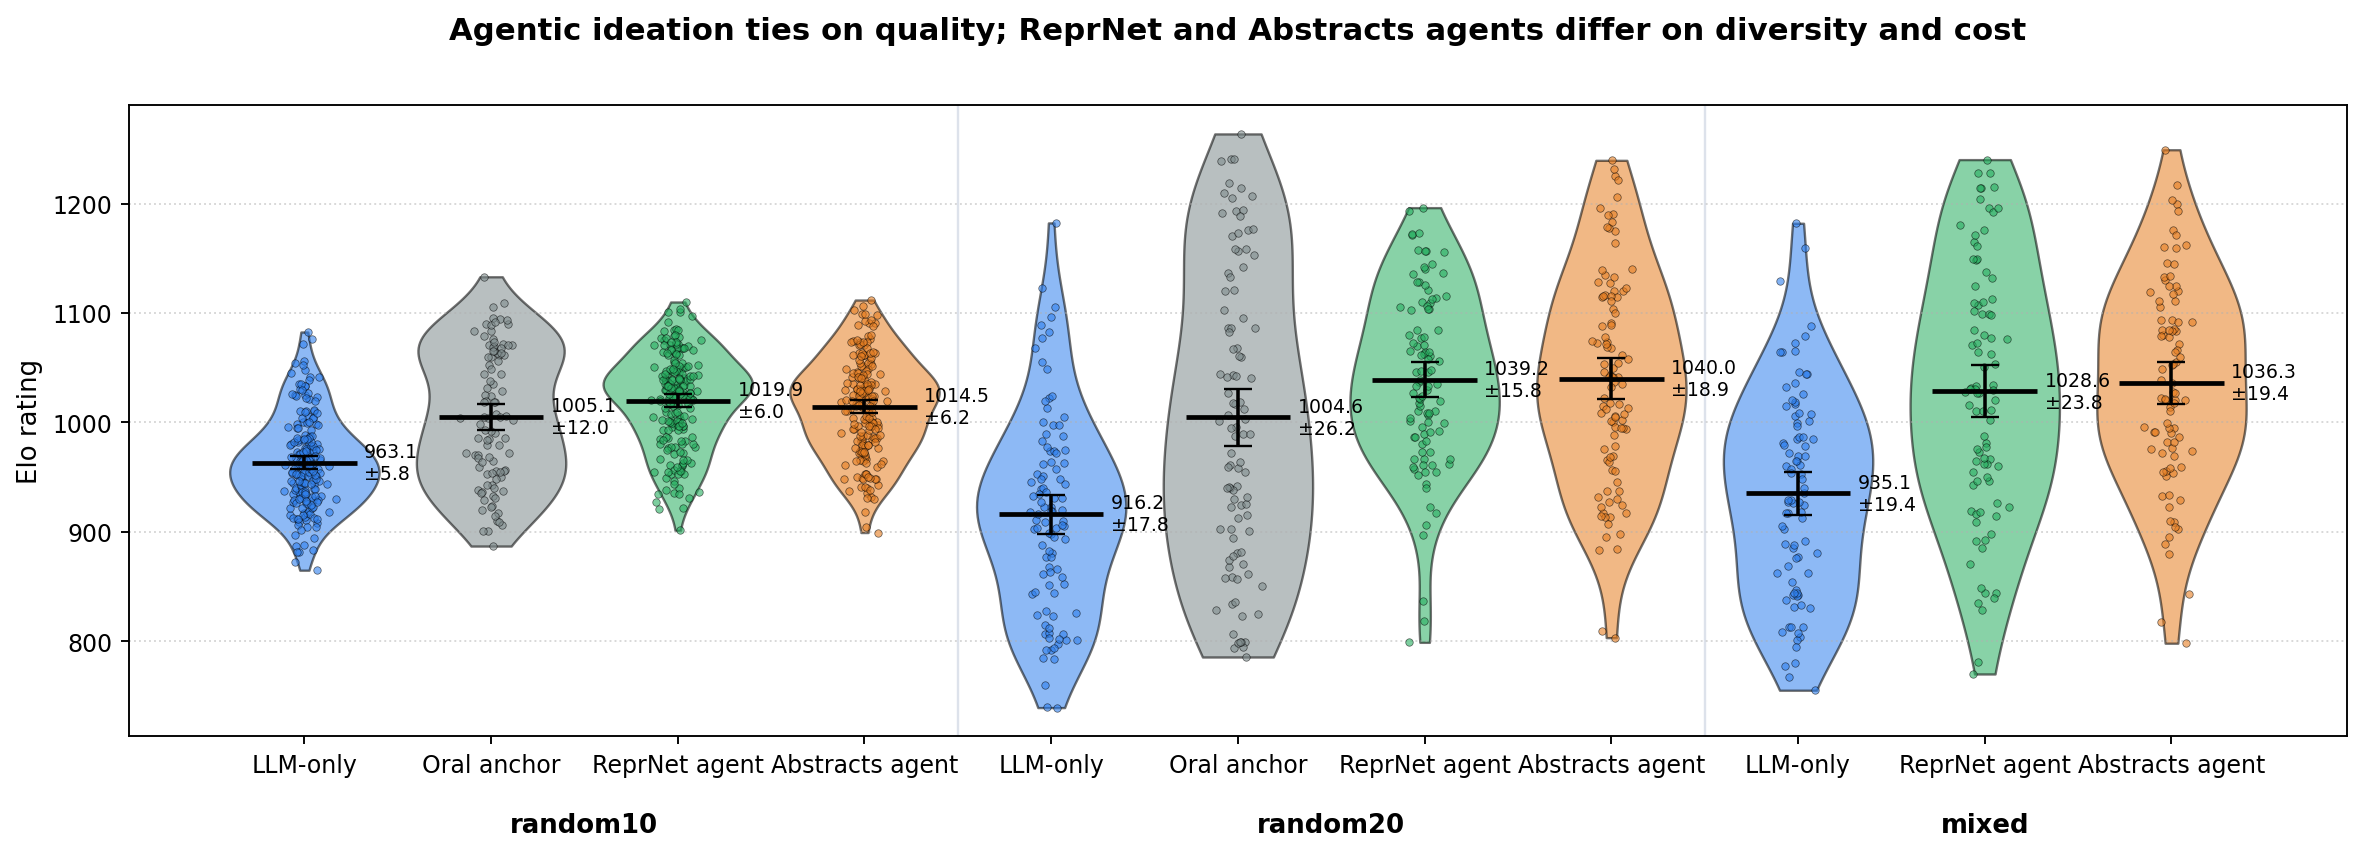
\includegraphics[width=0.92\textwidth]{figures/fig_quality.png}
  \caption{Per-idea Elo distributions by setting and arm.  Both
  agentic arms (ReprNet and Abstracts agents) beat the shuffled LLM-only
  baseline by $+57$--$+123$ Elo and reach or exceed the ICLR 2026
  oral anchor in the within-domain settings; the ReprNet and Abstracts agents are
  visually and statistically tied within each tournament's noise
  floor (rms 5.8--8.2 Elo).  Each panel is one half-budget multi-way
  round-robin tournament (random10: 4-way / 1200 matches; random20:
  4-way / 2400 matches; Nature+ICLR mixed: 3-way / 1800 matches; no
  oral anchor for the mixed groups).  Numeric values match
  Table~\ref{tab:quality}.}
  \label{fig:quality}
\end{figure*}

\begin{table*}[t]
\centering
\small
\setlength{\tabcolsep}{4pt}
\begin{tabular}{lrrrrrrr}
\toprule
Setting & LLM-only & ReprNet & Abstracts & Anchor & ReprNet$-$LLM-only & Abstr$-$LLM-only & ReprNet$-$Abstr \\
\midrule
Random10 ICLR        & 963.11 & 1019.88 & 1014.46 & 1005.10 & $+56.77$ & $+51.35$ & $+5.42$ \\
Random20 ICLR        & 916.22 & 1039.22 & 1039.99 & 1004.57 & $+123.00$ & $+123.77$ & $-0.77$ \\
Nature+ICLR mixed    & 935.07 & 1028.59 & 1036.34 &   ---   & $+93.52$ & $+101.27$ & $-7.75$ \\
\bottomrule
\end{tabular}
\caption{Quality results from the half-budget multi-way tournaments
(random10: 4-way, 1200 matches; random20: 4-way, 2400 matches; mixed:
3-way, 1800 matches).  All Elo values within a setting are on a
single common scale because they are rated against each other in the
same tournament.  Anchor Elo is the mean Elo of 100 ICLR 2026 oral
ideas when included.  Each LLM-only and ReprNet-agent pool contains
90--200 ideas; Abstracts-agent pools contain 200/100/90 at
random10/random20/mixed.
Tournament rms convergence is $5.8$/$7$/$8.2$ Elo respectively.}
\label{tab:quality}
\end{table*}

\subsection{The ReprNet Substrate Wins Diversity, Largest Cross-Domain}

Although the ReprNet and Abstracts agents are tied on quality, the ReprNet agent wins
on local diversity in every setting (Table~\ref{tab:diversity}).  At
random10, ReprNet $D = 5.62 \pm 0.22$ vs Abstracts agent $D = 4.75 \pm 0.26$
(gap $+0.87$); at random20, $6.85 \pm 0.16$ vs $6.58 \pm 0.18$ (gap
$+0.27$); at the Nature+ICLR mixed setting, $6.38 \pm 0.20$ vs
$5.09 \pm 0.26$ (gap $+1.29$).  The largest ReprNet diversity edge thus
occurs in the cross-domain regime, where every idea must bridge an
unfamiliar source pair; the smallest occurs at random20, where the
20-paper source context already gives both agents broad raw material.
All three ReprNet-vs-Abstracts gaps exceed the combined 95\% CIs, so the
diversity edge survives similarity-judge noise.

The diversity advantage also distinguishes the ReprNet agent from a graph-free
control of the agentic loop.  LLM-only vs Abstracts agent gaps ($+0.47$,
$+0.27$, $+0.72$ respectively at random10, random20, mixed) confirm
that some of the diversity gain comes from the agentic loop alone---an
iterating agent samples a wider idea space than a single LLM-only call---but
the remaining ReprNet-over-Abstracts edge ($+0.87$, $+0.27$, $+1.29$) is
larger still, especially cross-domain, and is the cleanest evidence in
this paper for a genuine contribution of explicit graph structure
beyond agency.

\begin{table*}[t]
\centering
\small
\setlength{\tabcolsep}{4pt}
\begin{tabular}{lcccc}
\toprule
Setting           & LLM-only $D$     & Abstracts $D$    & KGAgent $D$      & ReprNet $D$ \\
\midrule
Random10 ICLR     & 4.28 $\pm$ 0.24 & 4.75 $\pm$ 0.26 & 5.09 $\pm$ 0.25 & \textbf{5.62 $\pm$ 0.22} \\
Random20 ICLR     & 6.31 $\pm$ 0.21 & 6.58 $\pm$ 0.18 & 6.68 $\pm$ 0.19 & \textbf{6.85 $\pm$ 0.16} \\
Nature+ICLR mixed & 4.37 $\pm$ 0.29 & 5.09 $\pm$ 0.26 & 5.81 $\pm$ 0.27 & \textbf{6.38 $\pm$ 0.20} \\
\bottomrule
\end{tabular}
\caption{Diversity score $D = 10 -$ average nearest-neighbor LLM
similarity; the highest score per setting is in bold.  Intervals are
95\% confidence intervals on the mean, computed as $\pm 1.96 \cdot
\mathrm{SEM}$ over the per-pair similarity ratings ($n = 240$ pairs
per arm at random10/random20; $n = 289$--$314$ at the mixed
setting).  All three ReprNet-vs-Abstracts gaps ($+0.87$, $+0.27$,
$+1.29$) clear the combined CI widths, so the ReprNet-agent diversity
edge over the Abstracts agent is statistically real in every
setting, with the largest effect in the cross-domain mixed regime.
KGAgent (generic-knowledge-graph ablation) sits between the Abstracts
agent and ReprNet in all three settings ($5.09$, $6.68$, $5.81$ vs
ReprNet's $5.62$, $6.85$, $6.38$), confirming that ReprNet's typed
Repr/Transform schema adds a real $+0.17$ to $+0.57$ diversity gain
on top of whatever generic structured graph would buy, with the
largest effect in the cross-domain mixed regime.  At random20 a
finer-grained ablation (NR: typed Repr/Transform but no realization
edges) drops diversity to $6.30 \pm 0.21$, below the generic KG's
$6.68$ and barely above the LLM-only baseline's $6.31$, showing the
realization hierarchy carries almost all of the diversity edge.}
\label{tab:diversity}
\end{table*}

The interdisciplinary rubric corroborates the Elo and diversity results,
locating the gain in integration rather than in surface domain coverage
(Table~\ref{tab:rubric}).  The ReprNet agent improves four of the five
axes, with the largest movements in integration depth (4.23$\to$4.41) and
bidirectional value (3.93$\to$4.12)---both of which target whether the
domains genuinely shape each other, rather than whether both happen to be
mentioned.  Feasibility rises only marginally (2.64$\to$2.73), so neither
representation has yet solved the well-known feasibility gap.  Source
grounding decreases modestly (4.32$\to$4.09), revealing an interpretable
trade: graph-conditioned ideas synthesize more deeply across sources but
attribute back to specific abstracts less explicitly than direct
prompting.

\begin{table}[t]
\centering
\small
\begin{tabular}{lrr}
\toprule
Rubric axis & LLM-only & ReprNet \\
\midrule
Domain coverage & 4.90 & 4.97 \\
Integration depth & 4.23 & 4.41 \\
Bidirectional value & 3.93 & 4.12 \\
Source grounding & 4.32 & 4.09 \\
Feasibility & 2.64 & 2.73 \\
\bottomrule
\end{tabular}
\caption{Interdisciplinary rubric means on a 1--5 scale.}
\label{tab:rubric}
\end{table}

\subsection{Quality--Cost Tradeoff}

The agentic quality gain comes at a 43--95$\times$ generation-token
premium over the shuffled LLM-only baseline, concentrated in input-side
traversal context rather than output length (Table~\ref{tab:gencost}; full per-step totals in
Appendix~\ref{app:method-details}, Table~\ref{tab:stepcost}).
Per-idea generation tokens for the ReprNet agent are 282.8k, 380.4k, and
271.8k in random10, random20, and mixed, against 3.0k, 5.4k, and 6.3k
for the LLM-only baseline.  Disaggregating by call type shows that this
multiplier comes almost entirely from accumulated tool-call history and
graph-retrieval context, so the bottleneck is the size of the context
the agent reasons over, not the length of the ideas it writes.

The Abstracts agent sharpens what kind of agentic context is cheap and
what kind is expensive, now across all three benchmarks.  Under the
matched 50 tool-call / 70 request budget shared with the ReprNet agent,
Abstracts agent consumes 476.1k, 490.5k, and 486.1k tokens per idea at
random10, random20, and Nature+ICLR mixed respectively---in every case
\emph{more} than the ReprNet agent's 282.8k / 380.4k / 271.8k while
reaching statistically identical mean Elo (Table~\ref{tab:gencost}).
Per-call counts are nearly identical across the two agentic arms
($\sim 30$--$36$ requests per idea), so the cost difference is not a
count-of-calls difference; it is a payload difference.  Each
\texttt{read\_paper}, \texttt{search\_papers}, or \texttt{bridge}
return carries one or more full paper abstracts back into the agent's
context, whereas the graph tools (\texttt{get\_node},
\texttt{find\_paths}, etc.) typically return a handful of CamelCase
node names and short descriptions, so the per-call payload is roughly
an order of magnitude smaller on the graph substrate.

The cost advantage of the ReprNet agent is consistent and largest cross-domain.
The Abstracts/ReprNet ratio is 1.68$\times$ at random10, 1.29$\times$ at
random20, and 1.79$\times$ at Nature+ICLR mixed---the same regime where
the ReprNet agent also delivers its largest diversity edge.  Across the three
benchmarks combined, the ReprNet agent saves on the order of $130$--$200$k
tokens per idea at matched quality.  In other words, the ReprNet agent's value
under matched-quality comparison is not better mean Elo but
(i) better local diversity, and (ii) the ability to deliberate over a
compact symbolic substrate rather than re-reading raw abstracts every
time the agent wants to look something up.

This cost structure positions two follow-on directions.  First,
traversal-context compression for the ReprNet agent---cached subgraph
summaries, sparser retrieval, principled early stopping---remains the
highest-leverage way to bring the absolute token premium down further.
Second, for any non-graph agentic baseline, the natural symmetric move
is retrieval over distilled paper representations (titles, keyword
sets, or short autogenerated digests) rather than full abstracts,
which would make the comparison cleaner on the cost axis.  We did not
run the distilled Abstracts-agent variant in this paper.

\begin{table*}[t]
\centering
\small
\setlength{\tabcolsep}{4pt}
\begin{tabular}{lrrrrr}
\toprule
Setting & LLM-only & ReprNet & Abstracts & ReprNet/LLM-only & Abstracts/ReprNet \\
\midrule
Random10 ICLR        & 3.0k & 282.8k & 476.1k & 95.1$\times$ & 1.68$\times$ \\
Random20 ICLR        & 5.4k & 380.4k & 490.5k & 71.0$\times$ & 1.29$\times$ \\
Nature+ICLR mixed    & 6.3k & 271.8k & 486.1k & 43.0$\times$ & 1.79$\times$ \\
\bottomrule
\end{tabular}
\caption{Per-idea generation tokens by arm.  Each entry includes input
and output tokens for the full idea-generation call sequence
(excluding one-time graph construction).  Across all three benchmarks
the Abstracts agent consumes 1.29--1.79$\times$ more tokens per idea
than the ReprNet agent at statistically tied mean Elo; the gap is
largest in the cross-domain mixed setting, where the ReprNet agent's
symbolic substrate compresses paper content most aggressively.}
\label{tab:gencost}
\end{table*}

% Step-level token-usage table moved to Appendix A
% (Table~\ref{tab:stepcost}).

\subsection{Ablation: Typed Schema vs Generic Knowledge Graph}

The Abstracts agent comparison shows the agentic loop carries the
quality gap over the LLM-only baseline, but leaves open whether
ReprNet's residual diversity-and-cost edge comes from \emph{any}
structured graph at all or specifically from its Repr/Transform
typed schema (Repr = noun, Transform = verb, realization edges for
"is-a", typed input/output/composer edges).  To isolate the schema
contribution we run a third ablation across all three benchmarks:
\textbf{KGAgent}, a matched agent over a \emph{generic} knowledge
graph built by the same LLM at matched cost.  The generic KG
replaces ReprNet's two node types with a single untyped Entity
node and replaces typed edges with free-form string predicates
(e.g.\ \texttt{is\_a}, \texttt{uses}, \texttt{applies\_to},
\texttt{outputs}).  The KGAgent's tool palette mirrors ReprNet's
read-only graph tools, and per-idea token cost is matched to the
ReprNet ReprNet agent at every setting (random10: $283$k vs $282.8$k,
random20: $299$k vs $380$k --- KGAgent is actually \emph{cheaper}
here; mixed: $309$k vs $272$k tokens per idea, within $14\%$), so
quality differences cannot be attributed to budget.

To keep the comparison clean, the KG itself is built by an
\textbf{agentic} construction loop that mirrors ReprNet's per-paper
graph-build pipeline (\texttt{repr\_net.add\_content}): the same
LLM, a parallel multi-turn workflow, the same per-paper request
budget ($16$), and a parallel tool palette (\texttt{search\_entities},
\texttt{find\_entities}, \texttt{get\_entity},
\texttt{add\_triple}).  The only deliberate difference between the
two builders is the schema.  The resulting agentic-built KGs have
$72.5$ entities and $67$ edges on average (range $68$--$76$),
versus ReprNet's $\sim62$ nodes and $79$--$96$ edges --- a fair
size match.  We also report results for a non-agentic baseline KG
built by a single-shot extractor; that variant has $86.8$ entities
on average because its lack of cross-paper search produces less
entity reuse.

\begin{table*}[t]
\centering
\small
\setlength{\tabcolsep}{6pt}
\begin{tabular}{lrrrrrrr}
\toprule
Benchmark (build)        & KGAgent Elo & ReprNet Elo & $\Delta$Elo & rms   & $\approx\sigma$ & $\Delta D$ & cost k tok (KG\,/\,Repr) \\
\midrule
random10 (agentic)       & $980.33$    & $1019.67$   & $+39.34$    & $7.20$  & $5.5$ & $+0.53$ & $283.3\,/\,282.8$ \\
random10 (one-shot)      & $987.04$    & $1012.96$   & $+25.92$    & $7.05$  & ---   & ---     & ---               \\
random20 (agentic)       & $985.62$    & $1014.38$   & $+28.76$    & $10.47$ & $2.7$ & $+0.17$ & $298.7\,/\,380.4$ \\
Nature+ICLR (agentic)    & $981.27$    & $1018.73$   & $+37.46$    & $10.31$ & $3.6$ & $+0.57$ & $308.6\,/\,272.0$ \\
\bottomrule
\end{tabular}
\caption{Typed schema vs generic knowledge graph, head-to-head
2-way Elo across all three benchmarks.  $\Delta$Elo and $\Delta D$
are ReprNet minus KGAgent (positive favours the typed schema);
rms is the per-arm tournament noise and $\approx\sigma$ the gap in
noise units.  Per-idea cost is matched within $\leq 22\%$ and at
random20 the typed arm is the \emph{more} expensive one, ruling out
a budget confound.  The one-shot-built KGAgent row shows the effect
survives a change of construction methodology.}
\label{tab:schema-ablation}
\end{table*}

In head-to-head 2-way Elo tournaments against ReprNet, the
agentic-built KGAgent loses by $+28.76$ to $+39.34$ Elo across the
three settings (Table~\ref{tab:schema-ablation}): random10 $980.33$
vs $1019.67$ ($+39.34$, rms $7.20$, $\approx 5.5\sigma$); random20
$985.62$ vs $1014.38$ ($+28.76$, rms $10.47$, $\approx 2.7\sigma$);
Nature+ICLR mixed $981.27$ vs $1018.73$ ($+37.46$, rms $10.31$,
$\approx 3.6\sigma$).  All three gaps clear the tournament noise
floor.  At random10 we also report results for a non-agentic
one-shot-built KGAgent ($987.04$ vs $1012.96$, $+25.92$, rms
$7.05$): the gap stays $25$--$40$ Elo across both build variants,
so the typed-schema effect is robust to KG construction
methodology.  Diversity differences mirror the Elo gaps, with
ReprNet ahead by $+0.53$, $+0.17$, $+0.57$ at random10, random20,
mixed (Table~\ref{tab:diversity}), and the ReprNet vs KGAgent CIs
cleanly separated at random10 and mixed; the random20 gap is the
smallest because the 20-paper context already gives both agents
broad raw material.

\paragraph{Decomposing the schema: the realization hierarchy
carries most of the effect.}  The KGAgent ablation collapses two
schema mechanisms at once --- typed Repr/Transform nodes \emph{and}
the realization (is-a) edge class --- into a single generic-graph
arm.  To separate the two we run a third variant at random20,
called \textbf{NR} (No Realization), that keeps the
typed Repr/Transform nodes and their structural input / output /
composer edges but removes the realization edge class entirely
(builder cannot create abstraction edges, ideation agent cannot
navigate parents).  Construction is otherwise identical to the
KGAgent fair builder, and per-idea cost is matched at $338$k tokens
vs ReprNet's $380$k ($\approx 11\%$ cheaper).  In a $1200$-match
Elo tournament NR loses to ReprNet by $990.09$ vs $1009.91$
($+19.82$ Elo, rms $11.23$, $\approx 1.8\sigma$); diversity drops
to $D = 6.30 \pm 0.21$ --- \emph{below} even the KGAgent's $6.68$
and barely above the LLM-only baseline's $6.31$
(Table~\ref{tab:nr-decomp}).

\begin{table}[t]
\centering
\footnotesize
\setlength{\tabcolsep}{4pt}
\begin{tabular}{lrrr}
\toprule
random20 arm                  & $\Delta$Elo & $D$    & cost k tok \\
\midrule
LLM-only baseline               & ---         & $6.31$ & $5.4$      \\
KGAgent (generic, untyped)    & $+28.76$    & $6.68$ & $298.7$    \\
NR (typed, no realization)    & $+19.82$    & $6.30$ & $338.0$    \\
ReprNet (typed + realization) & ref         & $6.85$ & $380.4$    \\
\bottomrule
\end{tabular}
\caption{Decomposing the schema at random20.  $\Delta$Elo is the
gap to ReprNet (positive = ReprNet ahead).  Adding typed nodes back
(KGAgent$\to$NR) closes $\approx 31\%$ of the Elo gap; adding the
realization hierarchy back (NR$\to$ReprNet) closes the remaining
$\approx 69\%$ and recovers essentially all of the diversity.  NR's
$D=6.30$ falls \emph{below} the untyped KGAgent, isolating the
realization hierarchy as the source of ReprNet's diversity edge.}
\label{tab:nr-decomp}
\end{table}  Comparing within
the random20 setting, the Elo gap shrinks by $\approx 31\%$ when
realization is removed (from KGAgent's $+28.76$ to NR's $+19.82$),
so typed structural edges (composer / input / output) account for
about a third of the schema's Elo edge.  But diversity moves in the
opposite direction: removing realization \emph{hurts} diversity
more than removing typing did ($-0.55$ from ReprNet vs $-0.17$ for
KGAgent), pointing to the realization hierarchy as the source of
ReprNet's diversity advantage.  A plausible reading is that
KGAgent's free-form predicates accidentally include weak
abstraction-like relations (\texttt{is\_a}, \texttt{applies\_to},
\texttt{generalizes\_to}) that the agent can use as fall-back
abstraction navigation, whereas NR explicitly forbids any
abstraction edge of any kind and the agent gets stuck in local
structural neighbourhoods.  Together, the two ablations decompose
the schema effect into a structural-typing contribution (about a
third of the Elo gap) and a much larger realization-hierarchy
contribution (the rest of the Elo gap plus essentially all of the
diversity gap).

The typed schema therefore does measurable work beyond what any
matched-cost matched-build structured graph would buy, and the NR
decomposition pins down which part of the schema does it.  Three
mechanisms in ReprNet are absent from the generic KG:
\textbf{(i) Transform nodes give methods first-class identity}
rather than burying them as predicates on noun-noun pairs;
\textbf{(ii) typed $(in\_nodes, out\_nodes, composer)$ edges
expose method composition explicitly}, allowing the agent to
follow "method X composes method Y" without flattening into a
predicate chain; \textbf{(iii) realization edges form a clean
is-a hierarchy} distinct from other predicates, giving the agent
a separate axis for abstraction.  The NR ablation, which keeps
(i)+(ii) but removes (iii), shows that the abstraction hierarchy
of (iii) is the dominant mechanism: it carries roughly two thirds
of the Elo gap and essentially all of the diversity gap.  The
typed structural edges of (i)+(ii) still contribute the remaining
third of the Elo gap.  The consistency of the schema effect across
all three benchmarks --- both within-domain and cross-domain, and
robust to construction methodology --- together with this internal
decomposition is the cleanest evidence in this paper that the
schema, not the \emph{presence} of graph structure, is what gives
ReprNet its residual edge.

\clearpage

\section{Discussion}

The agentic-vs-LLM-only advantage is consistent enough across
benchmarks to rule out the usual confounders that complicate ideation
results.  The effect persists in three independently constructed
benchmarks, holds in both within-domain (random ICLR) and cross-domain
(Nature+ICLR) settings, and---unlike many ideation studies---survives
a deliberately strengthened baseline in which the LLM-only arm sees the
same source identities under deterministically reshuffled abstract
order.  Positional artifacts, source-pool drift, and differential
exposure cannot explain the agentic gain.

The calibrated scale places this advantage in a regime where it is
interpretable, not just statistically separated.  LLM-as-judge
protocols are noisy in absolute terms, yet the same protocol correctly
separates ICLR orals from posters by 66.0 and 35.1 Elo points across
two consecutive years; the agentic-vs-LLM-only gaps of $56.8$--$123.0$
Elo therefore exceed the calibrated reference gap by
$0.9$--$3.5\times$.  A margin of this size, together with concurrent
diversity gains and deeper integration on the interdisciplinary
rubric, supports reading the effect as a qualitatively different class
of ideas rather than a marginal stylistic improvement.

The Abstracts agent answers the natural follow-up question
cleanly.  Across all three settings, the ReprNet and Abstracts agents are
statistically indistinguishable on mean Elo (gaps of $+5.4$, $-0.8$,
and $-7.8$ Elo, each within its tournament rms), so the entire
agentic-vs-LLM-only gap is carried by the agentic loop itself rather
than by the representation graph.  This is a strong, falsifiable
finding: ablating away the graph at matched compute does not move
judged quality.  At the same time, the graph contributes a real and
consistent improvement on a different axis: nearest-neighbor diversity
is $+0.27$ to $+1.29$ higher under graph conditioning than under
Abstracts agent, with the largest effect in the cross-domain Nature+ICLR
setting and the smallest in the within-domain random20 setting.  The
graph also delivers this advantage at lower cost: Abstracts agent burns
$1.29$--$1.79\times$ more tokens per idea than the ReprNet agent at
matched quality.

The most useful way to interpret the cost--quality--diversity triangle
is therefore as follows.  The agentic loop is the right substrate for
LLM scientific ideation; one-shot prompting is not.  Within that
substrate, choosing a symbolic graph representation over re-reading
raw abstracts buys a consistent diversity bonus (largest where the
agent has to bridge unfamiliar domains) and a consistent token
discount (also largest cross-domain).  These effects are smaller in
absolute terms than the agentic-vs-LLM-only gap but more reliable across
settings, and they identify the regimes where explicit graph structure
is most worth investing in: cross-domain ideation and any setting
where local idea-base redundancy matters.  Conversely, in
within-domain settings where the source pool is already broad
(random20), the ReprNet agent buys little beyond cost efficiency, and a
well-tuned non-graph agent may be a perfectly adequate substitute.

Cost compression is therefore not just about reducing the agentic
arm's absolute token premium ($43$--$95\times$ over the LLM-only
baseline).  It is also about closing the Abstracts--ReprNet cost gap on
the symbolic side, e.g.\ through cached subgraph summaries, sparser
retrieval, and principled early stopping---and, symmetrically, on the
flat side through retrieval over distilled paper representations
rather than full abstracts.  Both directions sit on the
quality-equivalent Pareto frontier identified by this paper.

\section{Limitations}

Several limitations should temper the interpretation.
\textbf{(i) LLM-judged quality.}  All quality scores derive from LLM
judges; exceeding the oral anchor inside an LLM-judged tournament
should be read as a relative preference signal, not a claim that the
generated ideas would be accepted as oral papers.  Multi-judge
robustness has not yet been confirmed.
\textbf{(ii) Single generator.}  All ideas are generated by the same
underlying LLM; whether the agentic-loop dominance and the ReprNet
diversity edge transfer to other model families is open.
\textbf{(iii) Abstracts, not executed projects.}  The benchmarks
evaluate generated paper-style abstracts rather than experimentally
validated research projects.
\textbf{(iv) Sample size in the interdisciplinary setting.}  90 ideas
per arm at mixed yields wider intervals than the within-domain
random ICLR pools, even though the direction and ordering remain
consistent.
\textbf{(v) Persistent feasibility gap.}  Feasibility on the rubric
remains modest in both agentic arms ($2.6$--$2.7$ on a 1--5 scale),
suggesting that neither representation has solved the long-standing
feasibility weakness in LLM ideation.
\textbf{(vi) Cost.}  Even the cheaper agentic arm (graph) costs
$43$--$95\times$ more tokens per idea than direct prompting; production
deployment would require substantial optimization before the approach
is preferable in cost-sensitive scenarios.
\textbf{(vii) Half-budget multi-way Elo.}  Adding Abstracts agent doubled
the number of arms per tournament without doubling matches, leaving
tournament rms at $5.8$--$8.2$ Elo; some Abstracts-vs-ReprNet gaps
(e.g.\ $+5.4$ at random10) sit close to that noise floor.  Larger
tournaments would tighten the inference at the same qualitative
ordering.

\section{Reproducibility}

All experimental artifacts can be re-audited from the public layout under
\path{paper/} and \path{experiments/}.  Figures are authored as HTML and
matplotlib sources rendered by \path{paper/scripts/build_assets.py};
numeric tables are extracted from local experiment outputs into
\path{paper/data/results.json}; and the matched random benchmark can be
re-audited end-to-end with
\path{experiments/2026-05-12_iclr2025_random_fair_benchmark_v2/audit_benchmark.py
--strict}.  The cached graph-arm manifest records source network names,
duplicate names, and SHA-256 fingerprint verification for all 30 imported
graph groups, so any reproduction can independently confirm that no
protected graph was mutated during the experiments.

\section{Conclusion}

Letting El Agente Creativo operate iteratively over a fixed pool of
source papers yields measurably better and more diverse research ideas
than directly prompting the same LLM on the same papers, and the
agentic gain over the shuffled LLM-only baseline ($+56.8$ to $+123.0$
Elo across three benchmarks) exceeds a calibrated oral-vs-poster
quality scale by up to $3.5\times$, surpassing an ICLR 2026 oral
anchor on both within-domain random tournaments.  Comparing the ReprNet
agent against a matched non-graph agentic baseline (Abstracts agent) at every
setting splits this gain cleanly: the agentic loop carries
\emph{essentially all} of the quality lift over LLM-only (the ReprNet and
Abstracts agents are statistically tied at random10, random20, and mixed),
while explicit graph structure delivers two distinct, complementary
wins on top---a consistent nearest-neighbor diversity edge of $+0.27$
to $+1.29$ over Abstracts agent (largest cross-domain), and a
$1.29$--$1.79\times$ lower per-idea token cost at matched quality
(also largest cross-domain).  We therefore view agentic ideation as
the right substrate for LLM-based scientific discovery and explicit
graph structure over the literature as a consistent diversity-and-cost
win on top of it, most impactful in cross-domain settings.
Traversal-context compression and human-evaluation robustness are the
clearest next milestones toward practical deployment.

\section*{Acknowledgments}

We thank OpenReview and the ICLR community for hosting the
accepted-paper abstracts that form the within-domain benchmark, and
the Nature Research family of journals (Nature Physics, Nature
Biotechnology, Nature Chemistry) for the cross-domain source
material.  Source paper IDs, idea-base outputs, evaluation logs,
representation-graph fingerprints, per-call token usage, and the
Hugging Face dataset of all 39 source-paper groups are released under
the MIT license at the project repository for independent
verification and head-to-head benchmarking of future LLM idea
generators.

\clearpage
\onecolumn
\appendix

\section{Methodology Details and Reproducibility}
\label{app:method-details}

This appendix collects implementation-level details deferred from the
main text: the Bradley--Terry Elo update equations, the read-only
graph duplication protocol, the token-observability conventions, and
the per-step token-usage table.

\subsection{Bradley--Terry Elo update}

All ideas in a setting begin at Elo $R_i^{(0)} = 1000$.  Each Swiss
match contains $m=4$ ideas; the LLM judge returns a complete ranking
which is decomposed into all $m(m-1)/2$ ordered pairs.  For a pair
$(i,j)$ with current ratings $R_i$ and $R_j$, the Bradley--Terry
expected score \citep{bradley1952rank} and the rating update given the
pairwise outcome $S_i \in \{0,1\}$ are
\begin{equation}
  E_i = \frac{1}{1 + 10^{(R_j - R_i)/400}},
  \qquad
  R_i \leftarrow R_i + \frac{K}{m-1}(S_i - E_i),
\end{equation}
with $K = 32$.  Mean final Elo per arm is reported with nonparametric
bootstrap 95\% confidence intervals over idea-level Elo values.  The
same protocol is first run on the ICLR oral-vs-poster calibration sets
so every generated-idea gap can be read against a known-quality
reference scale.

\subsection{Read-only graph protocol}

Prior experiment graphs are treated as read-only artifacts so any
quality gain attributable to graph conditioning cannot be confounded
by silent graph mutation.  Each reuse of a cached graph proceeds in
three steps.  First, the source network is identified by name and a
SHA-256 fingerprint is computed over the canonicalized node and edge
payloads.  Second, the source is duplicated into an experiment-scoped
namespace (e.g.\ \texttt{reprgraph\_fair\_20260512\_v2\_*} for the V2
random ICLR benchmark, and
\texttt{reprgraph\_interdisciplinary\_20260512\_*\_augmented} for the
mixed benchmark's augmented copies); the duplicate's fingerprint is
recomputed and required to match the source.  Third, only the
duplicate is exposed to write operations (Nature-abstract insertion
in the mixed setting); the source remains untouched.  Source name,
duplicate name, and both fingerprints are logged in each experiment's
\texttt{cached\_graph\_arm\_manifest.json} so any reproduction can
independently confirm that no protected graph was mutated.

\subsection{Token observability}

Every generated idea and every judge call records normalized usage
fields \texttt{input\_tokens}, \texttt{output\_tokens},
\texttt{total\_tokens}, and \texttt{requests}.  OpenAI-compatible chat
completions are read from \texttt{response.usage}; Pydantic-AI
graph-construction runs are read from the native
\texttt{RunResult.usage()} object.  Per-idea usage is stored on each
idea JSONL row, and aggregate graph-build usage is additionally
attached to MongoDB network metadata.  Five expenditure categories
(graph construction, graph traversal, Elo judging, diversity judging,
and rubric judging) are tracked separately because their cost profiles
differ qualitatively; their per-step totals across the paper's
experiments are reported in Table~\ref{tab:stepcost}.

\begin{table*}[t]
\centering
\scriptsize
\setlength{\tabcolsep}{4pt}
\begin{tabular}{lrrrr}
\toprule
Step & In & Out & Total & Req. \\
\midrule
V2 LLM-only+ReprNet ideas (random10, random20) & 94.63M & 1.10M & 95.72M & 7891 \\
V2 Elo (random10, random20)               &  6.78M & 0.92M &  7.70M & 4000 \\
V2 diversity (random10, random20)         &  2.05M & 0.61M &  2.66M & 1932 \\
\textbf{Abstracts agent ideas (random10, n=200)} & \textbf{94.51M} & \textbf{0.71M} & \textbf{95.22M} & \textbf{7081} \\
\textbf{Abstracts agent ideas (random20, n=100)} & \textbf{48.69M} & \textbf{0.36M} & \textbf{49.05M} & \textbf{3532} \\
\textbf{Abstracts agent ideas (mixed, n=90)}     & \textbf{43.41M} & \textbf{0.33M} & \textbf{43.74M} & \textbf{3224} \\
Mixed augment          &  3.06M & 0.11M &  3.17M &  407 \\
Mixed LLM-only         &  0.51M & 0.06M &  0.57M &   90 \\
Mixed ReprNet          & 24.16M & 0.30M & 24.46M & 2391 \\
Mixed Elo              &  6.83M & 0.88M &  7.70M & 3533 \\
Mixed diversity        &  0.67M & 0.20M &  0.87M &  600 \\
Mixed rubric           &  0.12M & 0.06M &  0.18M &  183 \\
\bottomrule
\end{tabular}
\caption{Observed token usage by major step.  The three Abstracts-agent
rows cover 390 newly-generated ideas across the three benchmarks
(200+100+90); their combined cost is 188M tokens versus a roughly
estimated 110M for the ReprNet agent on the same idea counts, consistent
with the per-idea Abstracts/ReprNet ratios reported in
Table~\ref{tab:gencost}.}
\label{tab:stepcost}
\end{table*}

\subsection{Generic KG Ablation: Schema, Builder, Ideation, and Fairness}
\label{app:kg-ablation-impl}

This subsection collects the implementation details of the
generic-KG ablation reported in \S\ref{sec:results} and discusses
why each element is matched to the ReprNet agent.  The goal of
the ablation is to isolate a single variable --- the schema of the
substrate that the ideation agent reasons over --- so every other
degree of freedom must be controlled.  Three components define the
arm: the generic KG schema, the agentic per-paper KG construction
loop, and the KGAgent ideation agent.

\paragraph{Generic KG schema.}  ReprNet's substrate uses two node
types (Repr nouns and Transform verbs), a typed
$(\text{in\_nodes}, \text{out\_nodes}, \text{composer})$ tuple on
each Transform, and a dedicated \texttt{realization} edge class for
``is-a'' relations.  The generic KG removes all of these
distinctions.  It has a single untyped \texttt{Entity} node ---
any concept (data type, method, dataset, metric, etc.) is an
Entity --- and a single edge class carrying a free-form
\texttt{snake\_case} predicate string (e.g.\ \texttt{is\_a},
\texttt{uses}, \texttt{applies\_to}, \texttt{outputs},
\texttt{is\_evaluated\_on}, \texttt{improves\_upon},
\texttt{trained\_on}).  There is no fixed predicate vocabulary;
the builder LLM chooses whichever string it judges most apt for
each triple.  This is the standard generic knowledge-graph
representation and is what an off-the-shelf LLM would produce if
asked to ``extract a knowledge graph'' from a paper.  Crucially,
\emph{method composition collapses}: a Transform node with
$\geq 2$ inputs, $\geq 1$ output, and a composer in ReprNet
becomes a chain of $\geq 3$ generic predicates on noun-noun
pairs, losing first-class identity.  The hierarchy collapses too:
\texttt{realization} as a dedicated edge type becomes
\texttt{is\_a} as one predicate among many, which the agent must
disambiguate from \texttt{uses}, \texttt{applies\_to}, etc.
This collapse is the single variable under test.

\paragraph{Agentic construction loop.}  ReprNet's KG builder
(\texttt{repr\_net.add\_content}) processes one paper at a time
through a Pydantic AI agent that issues multiple tool calls per
paper, with a hard per-paper request budget of $16$ and a system
prompt that instructs the LLM to search first, reuse exact node
names where possible, and add only the central new nodes.  The
fair generic-KG builder (\texttt{kg\_builder\_agentic.py} in the
ablation experiment directories) mirrors this loop step-for-step:
the same generator LLM
(\texttt{aws/anthropic/bedrock-claude-sonnet-4-6}); the same
Pydantic AI driver with
\texttt{UsageLimits(request\_limit=16)}; the same workflow shape
in the system prompt (read the abstract, search first, decide
which existing entities to reference, add 5--7 triples per paper,
then verify); and the same cross-paper state object that
accumulates entities and triples across the group.  The only
documented difference between the two builders is which schema
they emit.  We additionally report results for a one-shot baseline
builder (single LLM call per paper returning 5--7 triples, no
cross-paper search) to expose how much of the ablation outcome
depends on the construction methodology; \S\ref{sec:results}
shows the typed-vs-generic gap is robust across both build modes.

\paragraph{Builder tool palette.}  The fair builder exposes five
tools, each a direct counterpart of a ReprNet builder tool:
\texttt{search\_entities(query, top\_k)} (embedding-based; mirrors
ReprNet's \texttt{search\_similar\_nodes}),
\texttt{find\_entities(pattern)} (substring; mirrors
\texttt{find\_nodes}),
\texttt{get\_entity(name)} (inspect node + adjacent triples;
mirrors \texttt{get\_node}),
\texttt{add\_triple(subject, predicate, object)} (mirrors
ReprNet's \texttt{add\_repr}/\texttt{add\_transform}/\texttt{add\_realization}
combined, since generic edges carry no type), and
\texttt{list\_recent\_additions} (book-keeping helper).  The
search tool uses the same embedding provider
(\texttt{text-embedding-ada-002} via NVIDIA's inference endpoint)
that the rest of the pipeline uses for similarity scoring.

\paragraph{Resulting KG sizes.}  At random10 the fair-built
generic KGs average $72.5$ entities and $67$ edges per group
(range $68$--$76$), versus ReprNet's $\sim62$ nodes and $79$--$96$
edges --- a close size match.  The one-shot baseline produces
larger but more redundant graphs ($86.8$ entities on average)
because its lack of cross-paper search reduces entity reuse; this
size gap is exactly what the agentic builder fixes.  At random20
and the mixed setting, the same per-paper budgets produce graphs
in the same per-paper-density regime; we deliberately do not
re-tune the budget across settings because the ReprNet builder
does not re-tune either.

\paragraph{KGAgent ideation agent.}  The downstream ideation
agent (\texttt{kg\_agent.py}) is constructed by direct parallel to
the ReprNet agent.  It uses the same generator LLM, the same
Pydantic AI framework, the same \texttt{IdeaProposal} Pydantic
output schema (single title + abstract field), the same
$50$-tool-call / $70$-request ideation budget (constants
\texttt{TOOL\_CALL\_LIMIT} and \texttt{REQUEST\_LIMIT} in the
experiment driver), and the same workflow shape in the
methodology prompt: pick random entities, inspect, explore
neighbours, find paths, optionally search at another abstraction
level, synthesize, self-critique.  The tool palette is the
read-only counterpart of the builder palette:
\texttt{random\_entity(min\_degree)},
\texttt{get\_entity(name)} (full view: predicates, in/out
neighbours, source papers),
\texttt{search\_entities(query, top\_k)},
\texttt{get\_neighbors(name)}, and
\texttt{find\_paths(src, dst)}.  Each of these has a one-to-one
ReprNet counterpart, so the agent's reasoning loop is structurally
identical; only the graph it queries differs.  For the mixed
benchmark the methodology prompt is the interdisciplinary variant
(must use one ML and one Nature-domain concept; explain how the
scientific mechanism shapes the ML representation), again
matched to the ReprNet agent.

\paragraph{Fairness gates.}  Table~\ref{tab:kg-fairness-gates}
enumerates every degree of freedom of the comparison and marks
which arm controls it.  All but one --- the schema --- are matched
by construction; the schema is the deliberate variable under
test.  Per-idea token cost is the most easily-confounding variable
and is reported in three places: random10 ($283.3$k for fair KG
vs $282.8$k for ReprNet, within $0.2\%$), random20 ($298.7$k vs
$380.4$k, KG is $22\%$ \emph{cheaper}), and mixed ($308.6$k vs
$272$k, $14\%$ more expensive).  In every case ReprNet's quality
edge cannot be attributed to spending more compute per idea: at
random20 the more expensive arm is the typed-schema one, and yet
KGAgent still loses by $+28.76$ Elo.  This rules out the standard
``maybe the better arm just had more budget'' confound.

\begin{table*}[t]
\centering
\small
\setlength{\tabcolsep}{4pt}
\begin{tabular}{lcc}
\toprule
Degree of freedom                                  & ReprNet                       & KGAgent (fair build)         \\
\midrule
Source paper IDs per group                         & V2 random / mixed             & verbatim copy                \\
Generator LLM (builder + ideator)                  & Claude Sonnet 4.6 (Bedrock)   & same                         \\
Pydantic AI framework + output schema              & \texttt{IdeaProposal}         & same                         \\
Ideation tool budget                               & $50$ tool calls, $70$ req     & same constants               \\
Ideation workflow shape                            & random$\to$inspect$\to$explore$\to$bridge$\to$synth$\to$critique & identical \\
Ideation tool palette (read-only)                  & random / get / search / neighbours / paths & one-to-one counterparts \\
Per-paper KG-build LLM + driver                    & Pydantic AI multi-turn        & same                         \\
Per-paper KG-build request budget                  & $16$ requests                 & same ($\texttt{request\_limit=16}$) \\
Builder tool palette                               & search / find / get / add (typed) & search / find / get / add (untyped) \\
Per-paper token budget                             & natural outcome of above      & matched within $\leq 14\%$   \\
\midrule
\textbf{Substrate schema (variable under test)}    & \textbf{Repr+Transform typed} & \textbf{Entity + free predicate} \\
\bottomrule
\end{tabular}
\caption{Fairness gates for the generic-KG ablation.  Every
degree of freedom is matched between the two arms except the
substrate schema, which is the variable under test.  The
``KGAgent (fair build)'' column refers to the agentic-built
generic KG used at every reported setting; \S\ref{sec:results}
additionally reports a one-shot-built variant at random10 to
verify that the typed-vs-generic effect is not an artifact of
how the KG was assembled.}
\label{tab:kg-fairness-gates}
\end{table*}

\paragraph{Why each gate matters.}  Each row of
Table~\ref{tab:kg-fairness-gates} closes a specific alternative
explanation for the observed gap.  Matching the source paper IDs
rules out content-pool differences.  Matching the generator LLM
rules out model-capability differences (e.g.\ one arm using a
stronger model).  Matching the Pydantic AI framework and
\texttt{IdeaProposal} schema rules out output-format effects
(JSON-validity rates, field-length nudges).  Matching the ideation
budget rules out ``more tool calls $\to$ better ideas''.  Matching
the workflow shape rules out prompt-engineering luck --- the same
inspect/explore/bridge/synthesize/critique scaffold is on both
sides.  Matching the tool palette one-to-one rules out
``ReprNet just exposes more affordances'': it does not; both
agents see five tools each, with matched semantics.  Matching the
construction loop (multi-turn agent with $\texttt{request\_limit=16}$
and search-first instructions) rules out the construction-quality
confound that motivated this ablation in the first place ---
without the agentic builder, the comparison would be against a
weaker one-shot generic KG and any quality gap could be blamed on
construction.  Matching the per-paper token budget closes the same
loophole at the cost level.

The single remaining systematic difference is therefore the
schema, and the empirical effect of that single difference
(Table~\ref{tab:diversity} and \S\ref{sec:results}) is a
$+28.76$ to $+39.34$ Elo gap and a $+0.17$ to $+0.57$ diversity
gap consistent across all three benchmarks.  Three concrete
schema mechanisms are absent from the generic KG and plausibly
account for the gap: Transform nodes give methods first-class
identity rather than burying them as predicates;
$(\text{in\_nodes}, \text{out\_nodes}, \text{composer})$ edges
expose method composition as a typed structural pattern rather
than a flattened predicate chain; and a dedicated
\texttt{realization} edge class gives the agent a clean
abstraction axis distinct from other predicates.  We discuss
which of the three carries which fraction of the gap as a
follow-on in \S\ref{sec:results}.

\subsection{Decomposition Ablation: Typed Schema Without Realization (NR)}
\label{app:nr-ablation}

The KGAgent ablation removes two ReprNet mechanisms at once: the
typed Repr/Transform node distinction \emph{and} the realization
(is-a) edge class.  To attribute the schema effect to one
mechanism or the other, we run an intermediate variant at
random20, \textbf{NR (No Realization)}, which
keeps the typed Repr/Transform node types and their structural
input / output / composer edges but \emph{forbids any realization
edge}.  The builder has \texttt{add\_repr} and \texttt{add\_transform}
tools (no \texttt{parent\_names} parameter), but no
\texttt{add\_parent} / \texttt{add\_realization} tool of any kind;
the ideation agent has no parent/child navigation tool.  All other
elements --- generator LLM, Pydantic AI driver, output schema,
multi-turn construction with $\texttt{request\_limit=16}$, ideation
budget ($50$ tool calls, $70$ requests), workflow scaffold ---
match the KGAgent fair builder and ideation agent one-to-one.  The
only systematic differences from ReprNet are (a) the absence of
realization edges in the substrate and (b) the absence of any
abstraction-navigation tool in the ideation agent.

The resulting NR networks average $114.6$ nodes per random20
group ($75.9$ Repr + $38.7$ Transform) and $142.8$ structural
edges (input $860$, output $472$, composer $96$, summed across
all ten groups), with $0$ realization edges by construction.
All $200/200$ papers are processed cleanly (no
\texttt{request\_limit} hits).  Per-idea cost is $338$k tokens,
$\approx 11\%$ cheaper than the ReprNet agent's random20 cost
($380$k) and $\approx 13\%$ more expensive than the random20
KGAgent ($299$k).

In the head-to-head Elo tournament against ReprNet random20
($1200$ matches), NR loses by $990.09$ vs $1009.91$ ($+19.82$
Elo gap, rms $11.23$, $\approx 1.8\sigma$).  Top-5\% pairwise
diversity yields $D = 6.30 \pm 0.21$ ($n=240$ pairs).  These
numbers, set against the KGAgent and full-ReprNet arms, are
collected in Table~\ref{tab:nr-decomp}.

The headline interpretation is that the gap from KGAgent to NR
(closing $\approx 31\%$ of the Elo gap by adding typing back) is
attributable to typed structural edges, while the gap from NR to
ReprNet (closing the remaining $\approx 69\%$ of the Elo gap and
$+0.55$ in diversity) is attributable to the realization
hierarchy.  In particular, removing realization \emph{below} the
generic-KG baseline on diversity ($6.30 < 6.68$) is the key
evidence: without realization the agent cannot find any
abstraction-level bridges, and NR is the only ablation in which
the agent has \emph{strictly less} ability to navigate
abstractions than even the free-predicate generic KG (whose
predicate vocabulary accidentally contains abstraction-like
relations such as \texttt{is\_a}, \texttt{applies\_to},
\texttt{generalizes\_to}).

\section{High-Elo Generated Idea Examples}

Table~\ref{tab:examples} gives representative high-Elo generated ideas from
the ReprNet agent in each benchmark.  The examples are selected from the final Elo
JSONL files and exclude the ICLR oral-anchor calibration rows.

\begin{table*}[t]
\centering
\scriptsize
\setlength{\tabcolsep}{3pt}
\begin{tabular}{p{0.13\textwidth}p{0.06\textwidth}p{0.21\textwidth}p{0.51\textwidth}}
\toprule
Setting & Elo & Title & Idea sketch \\
\midrule
Nature+ICLR mixed & 1437.2 & GFlowNet-Guided Cis-Regulatory Sequence Design from Plant MPRA Fitness Landscapes & Uses GFlowNets to design plant cis-regulatory sequences under massively parallel reporter assay feedback.  The proposal targets epistatic promoter design and explicitly frames diversity preservation as a way to avoid active-learning mode collapse. \\
Nature+ICLR mixed & 1399.7 & Rotation-Equivariant Graph Networks for Predicting Chiral Phonon Angular Momentum Transfer in Anharmonic Crystals & Connects rotation-equivariant graph neural networks with chiral phonon angular-momentum conservation.  The idea proposes predicting anharmonic phonon scattering and spin-lattice transfer more cheaply than first-principles perturbation calculations. \\
Random10 ICLR & 1237.4 & Memorization Asymmetry as a Privacy Risk Signal in Speculative Decoding & Treats the mismatch between draft-model and target-model memorization profiles in speculative decoding as a privacy signal.  The proposed test measures whether accepted and rejected token proposals reveal memorized training examples. \\
Random10 ICLR & 1229.1 & In-Context Simulation-Based Inference via Autoregressive Score Matching on Markovian Trajectories & Recasts causal Transformers as amortized simulation-based inference engines over Markovian trajectories.  The method would learn posterior estimation in context, reducing retraining when simulators or observations change. \\
Random20 ICLR & 1184.4 & Causally-Structured Sparse Attention for Doubly Robust Estimation from Continuous-Time Clinical Data & Builds sparse attention masks around temporal causal structure for treatment-effect estimation from ICU-style sensor streams.  The proposal links transformer nuisance estimation with g-computation and inverse-probability weighting constraints. \\
Random20 ICLR & 1182.0 & Mechanistic Reverse-Engineering of Selective State Space Models on Algorithmic Tasks & Extends mechanistic interpretability from transformer circuits to selective state-space models such as Mamba.  The idea asks whether SSM solutions to algorithmic tasks can be reverse-engineered into human-readable mechanisms and formal accuracy bounds. \\
\bottomrule
\end{tabular}
\caption{High-Elo examples from generated graph-conditioned ideas.  Elo values are final idea-level ratings from the corresponding tournament outputs.}
\label{tab:examples}
\end{table*}

\clearpage
\section{Prompt Templates}

This appendix records the natural-language prompt templates used by the LLM
steps in the experiments.  Runtime fields such as source abstracts, prior
titles, graph-tool results, and idea text are shown as bracketed placeholders.
Deterministic steps such as source sampling, embedding calls, graph
fingerprinting, and aggregation do not use natural-language prompts.

\subsection{Random ICLR LLM-only Baseline}
\begin{lstlisting}[style=promptbox]
System:
You are a research scientist generating new ML research ideas.
Propose one focused, feasible, high-impact idea for a small team.
Do not claim completed results. Do not copy an input paper.
Return valid JSON only.

User:
Method: [method]

[method note: random abstracts, embedding-diverse abstracts, or
embedding-similar abstracts; avoid merely averaging papers.]

Prior generated titles to avoid:
[last prior titles]

Source abstracts:
[paper title, keywords, and abstract blocks]

Return exactly:
{
  "title": "<short title under 20 words>",
  "abstract": "<150-250 word forward-looking paper-style abstract>"
}
\end{lstlisting}

\subsection{Nature+ICLR LLM-only Baseline}
\begin{lstlisting}[style=promptbox]
System:
You are a senior interdisciplinary AI researcher. Generate one focused,
feasible research idea that genuinely integrates machine learning with
a scientific mechanism, measurement, constraint, or data process from
the supplied Nature abstracts. Return valid JSON only.

User:
Method: [mixed group prompt method]

Prior generated titles to avoid:
[last prior titles]

Source abstracts:
[10 ICLR abstracts and 5 Nature abstracts in deterministic per-idea
shuffled order]

Rules:
- Use at least one ICLR source and at least one Nature source.
- Do not merely propose applying a generic model to a scientific dataset.
- The Nature-domain content must change the ML representation, objective,
  evaluation, theory, simulator, or training signal.
- Be specific enough for a small research team to start implementation.

Return exactly this JSON object:
{
  "title": "<short title under 20 words>",
  "abstract": "<180-260 word forward-looking paper-style abstract>",
  "cross_domain_connection": "<one sentence explaining the concrete bridge>",
  "source_ids_used": ["<ids used>"],
  "risks": "<main feasibility or evaluation risk>"
}
\end{lstlisting}

\subsection{Representation Graph Construction}
\begin{lstlisting}[style=promptbox]
System:
You are an expert at building representation networks. A representation network
models a scientific domain as a directed graph of Repr nodes
(representations / data types) and Transform nodes (processes that convert
representations).

Node types:
- Repr: a data type, concept, or artifact (noun), with name, optional
  description, refs, and parent names.
- Transform: a process that converts one or more Reprs into others (verb),
  with name, in_node_names, out_node_names, composer_names, optional
  description, refs, and parent names.

Workflow:
1. Read the abstract carefully to identify the paper's key concepts.
2. Search first with search_similar_nodes using several queries.
3. Reuse existing nodes when possible and add only needed new Repr and
   Transform nodes.
4. Add Repr nodes, then Transform nodes, then parent links.

Rules:
- Repr = noun; Transform = verb.
- Every Transform must have in_node_names, out_node_names, and composer_names.
- Reuse exact existing node names instead of creating duplicates.
- Set refs=[url] on the most central new node.
- Use CamelCase names.

Budgeted pilot constraints:
- For each paper, add only the core contribution.
- Add 2-4 central Repr nodes and 1-2 central Transform nodes.
- Prefer reusable abstractions over paper-specific duplicates.

User:
Add representations from the following paper to the network.

URL: [paper URL or source ID]
Abstract / Content:
[paper abstract]

Instructions:
1. Analyze the abstract to identify key concepts and contributions.
2. Use search_similar_nodes with multiple queries.
3. Add new Repr nodes first, then Transform nodes.
4. Use find_nodes to verify the new nodes exist.
\end{lstlisting}

\subsection{Graph-Conditioned Ideation}
\begin{lstlisting}[style=promptbox]
System / methodology:
You are a creative interdisciplinary researcher generating ideas from a
representation graph that combines ICLR 2025 machine-learning papers with recent
Nature papers.

Your idea must:
- Use at least one machine-learning concept and at least one Nature-domain
  concept.
- Mechanistically integrate the domains; do not merely apply a generic model
  to a scientific dataset.
- Explain how the scientific mechanism, measurement, data process, or
  constraint changes the ML representation, objective, evaluation, simulator,
  or theory.
- Be feasible for a small research team in 6--12 months.
- Prefer ideas that can be evaluated using available scientific data,
  simulations, or controlled benchmarks.

Fixed workflow appended by the agent runner:
1. Pick random nodes using get_random_node.
2. Inspect the most interesting pair with get_node.
3. Explore parents and children briefly.
4. Find paths between nodes using find_paths or find_shortest_path.
5. Optionally search at another abstraction level.
6. Synthesize one research idea that bridges concrete nodes through a
   surprising connection.
7. Self-critique for feasibility, focus, reviewability, and natural language.

Task:
Generate a novel, feasible and impactful research idea by exploring the graph
of representations. Pick random nodes, explore hierarchy, find paths for
inspiration, then synthesize and self-critique before returning the final idea.

Output:
title: short descriptive title under 20 words.
abstract: one paragraph, 150-300 words, with problem, approach, specific
algorithms/datasets/metrics, expected contribution, and impact. Do not include
tool traces or internal graph node names.
\end{lstlisting}

\subsection{Elo Preference Judge}
\begin{lstlisting}[style=promptbox]
System:
You are an expert research evaluator with deep knowledge of machine learning,
chemistry, and materials science. You will be given several research ideas and
must rank them from most interesting and promising to least. Prioritise ideas
that are genuinely novel, scientifically exciting, concretely actionable by a
small team in 6-12 months, and high-impact. Respond with valid JSON only.

Do NOT reward number of cited papers, author-year references, length or polish
of the abstract, or incremental extensions without a fresh angle.

User:
Rank the following [n] research ideas from most promising (rank 1) to least
promising (rank [n]).

Idea 1:
[title and abstract, truncated at 2000 characters]

...

Output ONLY valid JSON:
{
  "ranking": [<list of idea numbers from best to worst>],
  "reasoning": "<2-3 sentences>"
}
\end{lstlisting}

\subsection{Diversity Similarity Judge}
\begin{lstlisting}[style=promptbox]
System:
You are an expert research analyst. Given two research ideas, rate how similar
they are in terms of core topic, methodology, problem formulation, and
potential applications. A score of 10 means the ideas are essentially the same
concept with minor wording differences. A score of 1 means they are completely
unrelated. Respond with valid JSON only.

User:
Rate the similarity between these two research ideas.

Idea A:
[title and abstract, truncated at 2000 characters]

Idea B:
[title and abstract, truncated at 2000 characters]

Rate their similarity from 1 (completely unrelated) to 10 (essentially
identical). Consider: core problem, methodology, target domain, and potential
applications.

Output ONLY valid JSON:
{
  "similarity_score": <1-10 integer>,
  "overlap_areas": "<brief description of what the ideas share>",
  "difference_areas": "<brief description of key differences>",
  "reasoning": "<2-3 sentence explanation of the similarity rating>"
}
\end{lstlisting}

\subsection{Interdisciplinarity Rubric Judge}
\begin{lstlisting}[style=promptbox]
System:
You are a strict research-program evaluator. Score interdisciplinary
AI+science ideas using only the provided title and abstract. Return valid
JSON only.

User:
Idea title: [title]

Idea abstract:
[abstract]

Score each field from 1 (weak) to 5 (excellent):
- domain_coverage: substantively uses both AI/ML and Nature-domain science.
- integration_depth: domains interact mechanistically rather than superficially.
- bidirectional_value: contributes to ML methodology and the scientific domain.
- source_grounding: appears grounded in supplied paper mechanisms, not generic.
- feasibility: executable by a small team in 6--12 months.

Return JSON:
{
  "domain_coverage": <1-5>,
  "integration_depth": <1-5>,
  "bidirectional_value": <1-5>,
  "source_grounding": <1-5>,
  "feasibility": <1-5>,
  "rationale": "<brief explanation>"
}
\end{lstlisting}

\clearpage
\twocolumn

\bibliographystyle{plainnat}
\bibliography{references}

\end{document}
